\section{Infrastructure DevOps et observabilité}
\label{chap:devops}

Cette section décrit la couche qui déploie, teste en continu et supervise les services présentés aux sections~\ref{chap:etl}, \ref{chap:webapp} et~\ref{chap:ia_rag}. Elle pose les conditions matérielles de l'hypothèse de frugalité H1 (\texttt{ENF-FRUG-01}) et réalise le volet infrastructure de \texttt{ENF-DISP-02} (disponibilité), \texttt{ENF-SEC-04}/\texttt{05} (audit, TLS), \texttt{ENF-MAINT-02} (tests en intégration continue) et \texttt{EF-ADM-03} (sauvegarde). Le chiffrage du coût réel et la validation de H1 relèvent de la section~\ref{chap:impact_metier}.

\subsection{Conteneurisation et déploiement mono-hôte}
\label{sec:devops_conteneurisation}

La vue de déploiement de la section~\ref{chap:architecture} (Figure~\ref{fig:deploiement}) situe l'infrastructure : tous les services tournent sur le serveur dédié décrit au §\ref{sec:env_realisation}, loué 30,23~USD par mois. Nous citons ce montant comme donnée de conception qui justifie le choix mono-hôte de l'ADR-03 (\S\ref{sec:adr}) ; sa confrontation au seuil de \texttt{ENF-FRUG-01}, avec les autres postes de coût, relève de la section~\ref{chap:impact_metier}.

Docker Engine orchestre l'ensemble sur un réseau unique, \texttt{soyaff\_network}. Chaque conteneur ne publie ses ports que sur \texttt{127.0.0.1} : ni la base PostgreSQL, ni l'API RAG, ni Airflow ne sont atteignables autrement que depuis le serveur lui-même. Quatorze conteneurs tournent en permanence, répartis en trois fichiers \texttt{docker compose} versionnés : la pile IA/ETL et la supervision dans le dépôt \texttt{assistant-soyaff}, l'application dans le dépôt \texttt{assistant-soyaff-app}. Le Tableau~\ref{tab:inventaire_conteneurs} les regroupe par plan fonctionnel.

\begin{table}[htbp]
\centering
\footnotesize
\caption{Inventaire des conteneurs de production, par plan fonctionnel (état au 27~septembre~2026)}
\label{tab:inventaire_conteneurs}
\begin{tabularx}{\linewidth}{|l|>{\raggedright\arraybackslash}p{5.5cm}|>{\raggedright\arraybackslash}X|}
\hline
\rowcolor[HTML]{EFEFEF}
\textbf{Plan} & \textbf{Conteneurs} & \textbf{Rôle} \\ \hline
Applicatif & \texttt{soyaff\_frontend}, \texttt{soyaff\_backend} & SPA React servie par un Nginx conteneurisé (\S\ref{sec:webapp_architecture}) ; API REST Express \\ \hline
Données & \texttt{soyaff\_postgres} & Moteur relationnel et vectoriel unique (PostgreSQL~16 + pgvector), mutualisé entre l'application, l'ETL et le RAG (ADR-04) \\ \hline
IA~/~RAG & \texttt{soyaff\_rag\_api}, \texttt{ollama} & Service FastAPI du chemin local (section~\ref{chap:ia_rag}) ; inférence Mistral~7B \\ \hline
ETL & \texttt{soyaff\_airflow\_web}, \texttt{airflow\_scheduler} & Interface et ordonnanceur du pipeline d'ingestion (section~\ref{chap:etl}, ADR-01) \\ \hline
Automatisation & \texttt{soyaff\_n8n} & Orchestrateur du routage hybride (ADR-02) \\ \hline
Supervision & \texttt{soyaff\_prometheus}, \texttt{soyaff\_node\_exporter}, \texttt{soyaff\_blackbox}, \texttt{soyaff\_loki}, \texttt{soyaff\_promtail}, \texttt{soyaff\_grafana} & Métriques et sondes (exportateurs~$\rightarrow$~Prometheus), journaux (Promtail~$\rightarrow$~Loki), tableaux de bord et alertes (Grafana), \S\ref{sec:devops_observabilite} \\ \hline
\end{tabularx}
\end{table}

Deux composants tournent hors de Docker. Un Nginx installé sur le serveur reçoit tout le trafic sur les ports~80 et~443 et le route par sous-domaine (\texttt{api.}, \texttt{n8n.}, \texttt{airflow.}, \texttt{monitor.soyaff-logstique.com}) vers le port local du conteneur concerné. Le \textit{runner} GitLab, service système, exécute les pipelines (\S\ref{sec:devops_cicd}). Le pare-feu \texttt{UFW} n'ouvre que les ports~22 (SSH), 80 et~443 (\S\ref{sec:devops_securite}).

Cette topologie mono-hôte, entièrement open source, rend la frugalité possible : c'est une \emph{condition} de H1, pas un résultat établi ici. Sa contrepartie est le point de défaillance unique assumé à l'ADR-03 : une panne du serveur arrête tous les services à la fois. Ce compromis est repris à la section~\ref{chap:discussion}.

\subsection{Intégration et déploiement continus (CI/CD GitLab)}
\label{sec:devops_cicd}

Les deux dépôts sont hébergés sur GitLab.com. Nous avons installé sur le serveur un \textit{runner} dédié, à \textit{executor} \texttt{shell}, qui exécute chaque job directement sur le serveur (Figure~\ref{fig:ops_runner}). C'est cohérent avec le mono-hôte de l'ADR-03 : les jobs de déploiement agissent sans intermédiaire sur les conteneurs de production. La contrepartie est qu'un job mal isolé pourrait, en principe, affecter le serveur lui-même.

\begin{figure}[H]
    \centering
    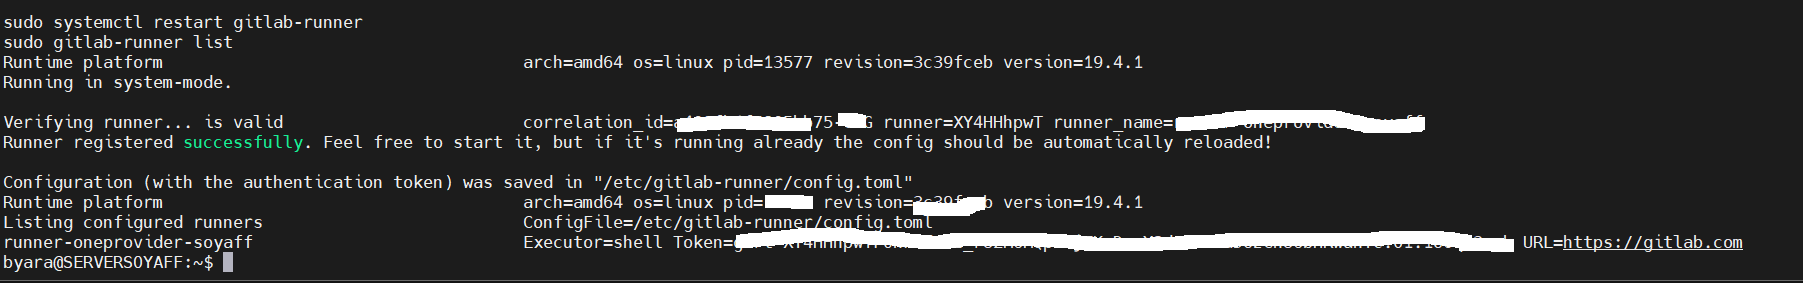
\includegraphics[width=0.9\textwidth]{figures/captures/ops_runner.png}
    \caption{Enregistrement du \textit{runner} GitLab sur le serveur de production}
    \label{fig:ops_runner}
\end{figure}

Deux dépôts, deux pipelines indépendants : \texttt{assistant-soyaff} porte la pile Python (ETL, RAG, supervision), \texttt{assistant-soyaff-app} l'application web. Leur ordre de déploiement est une contrainte opérationnelle : le second vérifie que le réseau \texttt{soyaff\_network}, créé par le premier, existe, et s'interrompt sinon.

\textbf{Des tests qui bloquent réellement.} Le Tableau~\ref{tab:cicd_jobs} détaille chaque job de test. Tous font échouer le pipeline en cas d'erreur, et un pipeline en échec ne déploie rien.

\begin{table}[htbp]
\centering
\footnotesize
\caption{Jobs de test des deux pipelines (état au 27~septembre~2026)}
\label{tab:cicd_jobs}
\begin{tabularx}{\linewidth}{|l|l|>{\raggedright\arraybackslash}X|>{\raggedright\arraybackslash}p{2.6cm}|}
\hline
\rowcolor[HTML]{EFEFEF}
\textbf{Job} & \textbf{Dépôt} & \textbf{Ce qu'il exécute} & \textbf{Couverture} \\ \hline
\texttt{test:python} & \texttt{assistant-soyaff} & Vérification de syntaxe des modules, puis \texttt{pytest} : 397 tests, dont des tests d'intégration contre un PostgreSQL~16 + pgvector jetable, démarré pour le job & 97,6~\% mesurés, plancher bloquant à 95~\% \\ \hline
\texttt{lint:backend}, \texttt{lint:frontend} & \texttt{assistant-soyaff-app} & ESLint et Prettier & sans objet \\ \hline
\texttt{test:backend} & \texttt{assistant-soyaff-app} & Jest : 122 tests unitaires et d'intégration contre une base de test & non mesurée en CI \\ \hline
\texttt{test:frontend} & \texttt{assistant-soyaff-app} & Vitest : 44 tests, puis construction de production & non mesurée en CI \\ \hline
\end{tabularx}
\end{table}

Les Figures~\ref{fig:ops_test_python}, \ref{fig:ops_test_backend} et~\ref{fig:ops_test_frontend} montrent ces trois suites en succès. Côté Python, nous avons fixé le plancher de couverture par cliquet : il est relevé à chaque progression mesurée, jamais abaissé.

\begin{figure}[H]
    \centering
    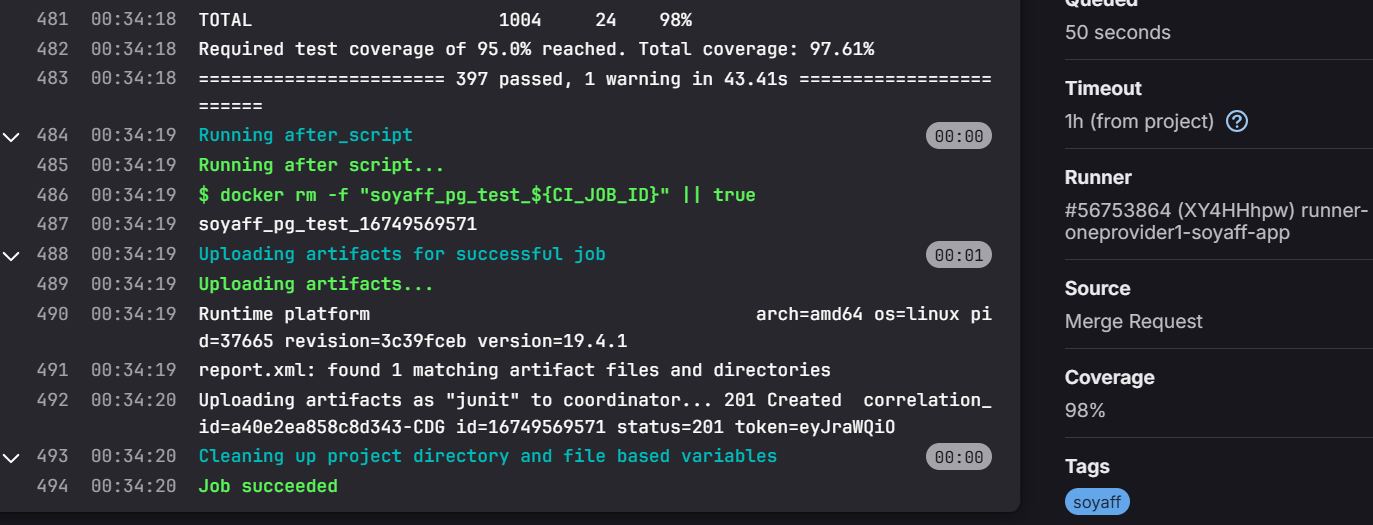
\includegraphics[width=0.7\textwidth]{figures/captures/ops_test_python.png}
    \caption{Job \texttt{test:python} : 397 tests réussis, couverture de 97,61~\% pour un plancher de 95~\%}
    \label{fig:ops_test_python}
\end{figure}

\begin{figure}[H]
    \centering
    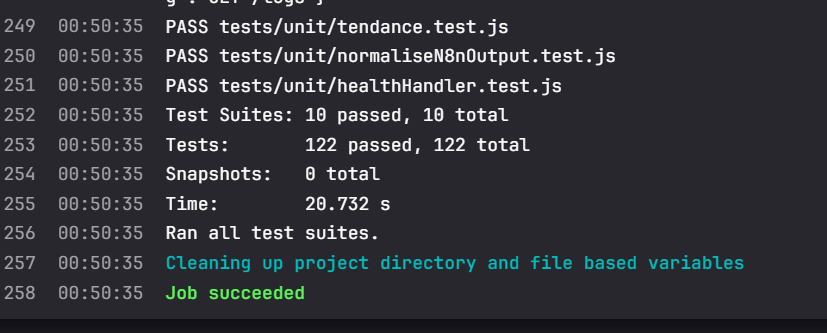
\includegraphics[width=0.5\textwidth]{figures/captures/ops_test_backend.png}
    \caption{Job \texttt{test:backend} : 122 tests réussis}
    \label{fig:ops_test_backend}
\end{figure}

\begin{figure}[H]
    \centering
    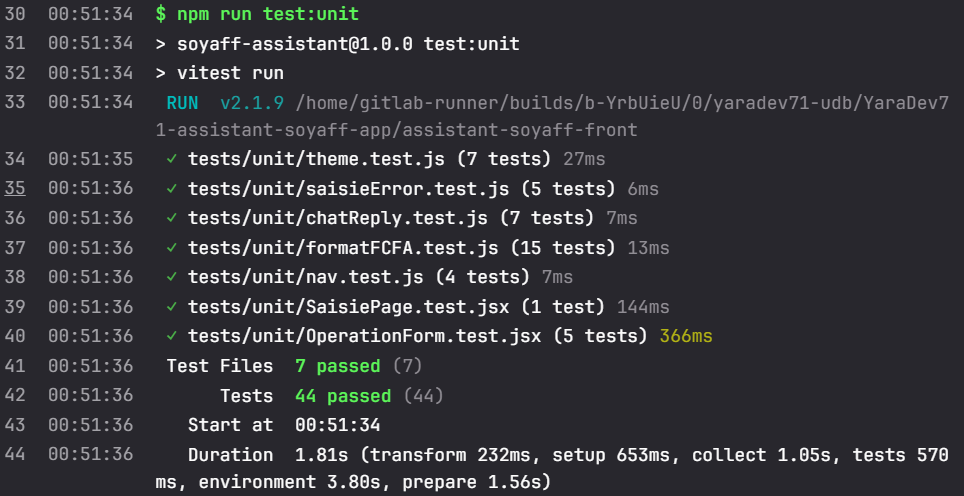
\includegraphics[width=0.55\textwidth]{figures/captures/ops_test_frontend.png}
    \caption{Job \texttt{test:frontend} : 44 tests réussis}
    \label{fig:ops_test_frontend}
\end{figure}

\textbf{Un déploiement automatique.} Les jobs \texttt{deploy:production} n'ont aucune validation manuelle : toute fusion sur \texttt{main} déploie. Le job récupère le code (\texttt{git reset --hard origin/main}), génère le fichier \texttt{.env} à partir des variables protégées de GitLab (aucun secret n'est écrit dans le dépôt), puis reconstruit et redémarre les conteneurs. Côté Python, il applique d'abord les migrations Alembic. Côté application, il interroge ensuite la sonde de santé du backend : si elle ne répond pas, le job échoue (Figure~\ref{fig:ops_deploy_app}). La Figure~\ref{fig:ops_pipelines} montre l'historique des pipelines : un job de test dure environ deux minutes et demie, un déploiement une trentaine de secondes.

\begin{figure}[H]
    \centering
    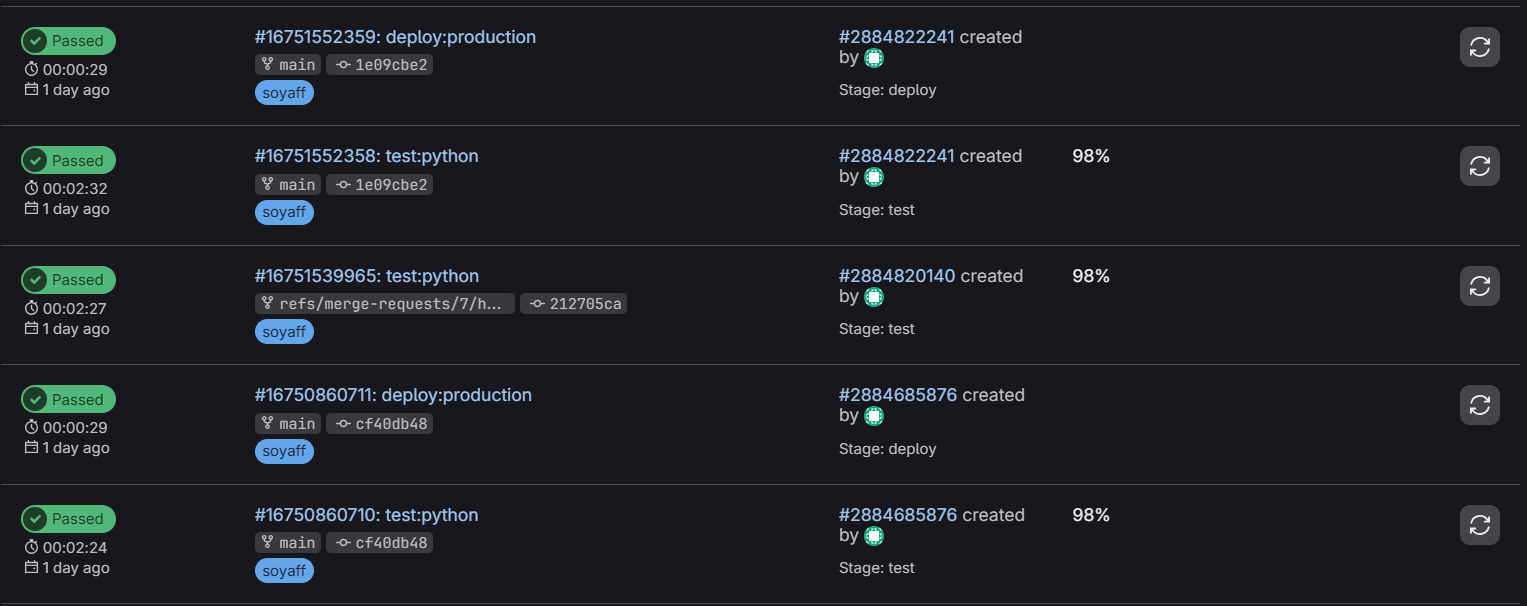
\includegraphics[width=0.85\textwidth]{figures/captures/ops_pipelines.png}
    \caption{Historique des jobs CI/CD : tests (couverture 98~\%) puis déploiement sur \texttt{main}}
    \label{fig:ops_pipelines}
\end{figure}

\begin{figure}[H]
    \centering
    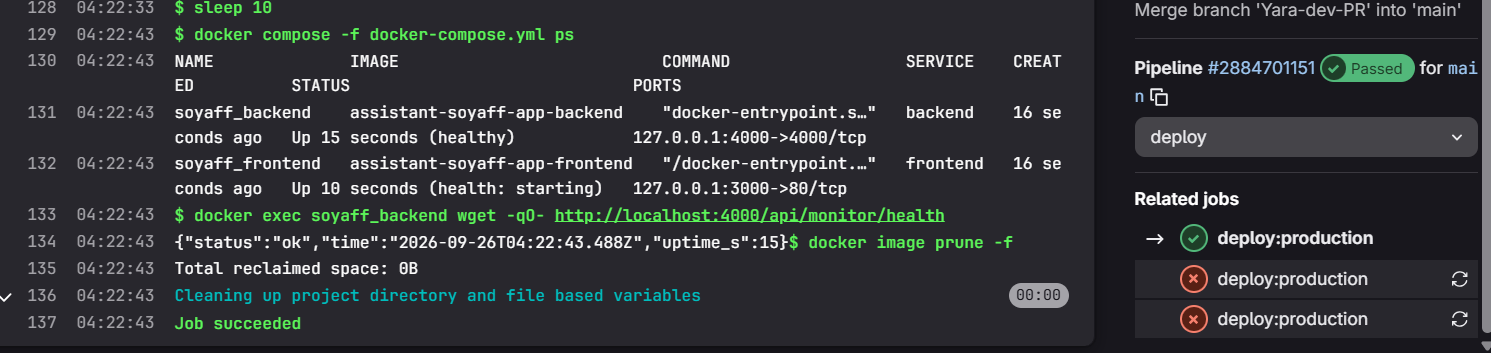
\includegraphics[width=0.85\textwidth]{figures/captures/ops_deploy_app.png}
    \caption{Déploiement automatique de l'application, vérifié par la sonde de santé du backend}
    \label{fig:ops_deploy_app}
\end{figure}

\begin{figure}[H]
    \centering
    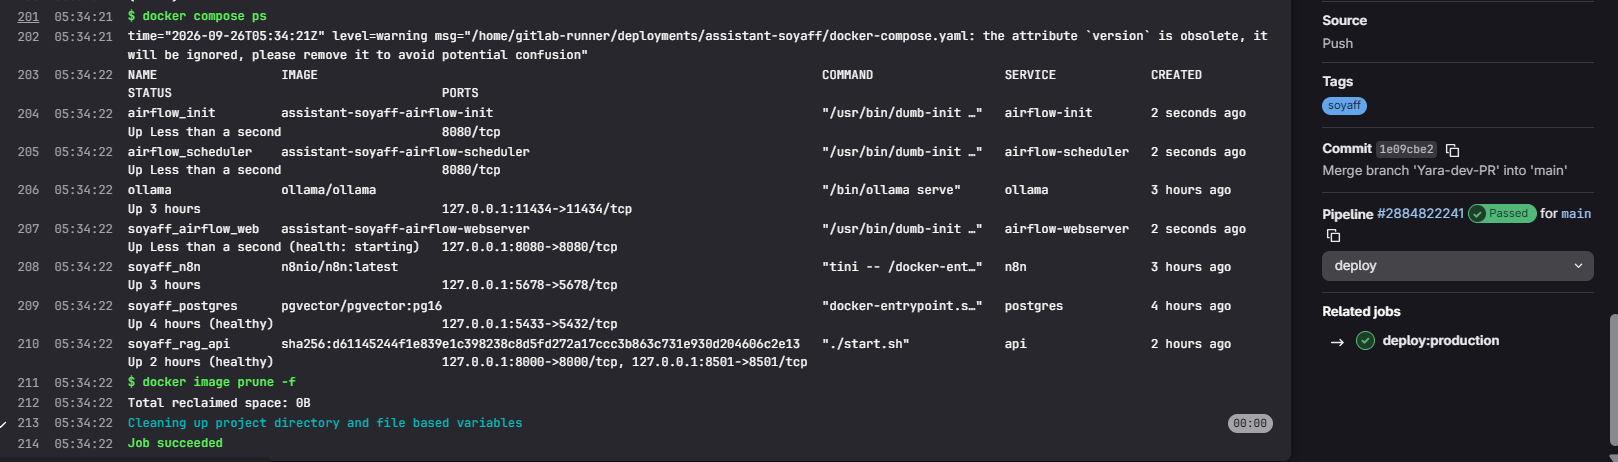
\includegraphics[width=0.85\textwidth]{figures/captures/ops_deploy_ia.png}
    \caption{Déploiement automatique de la pile IA/ETL : état des conteneurs en fin de job}
    \label{fig:ops_deploy_ia}
\end{figure}

Ce déploiement continu n'a pas de stratégie de bascule : ni \textit{blue-green}, ni retour arrière automatique. Côté Python, l'état des conteneurs affiché en fin de job (Figure~\ref{fig:ops_deploy_ia}) est informatif et ne fait pas échouer le job. Cette dette est reprise au \S\ref{sec:devops_dettes}.

\textbf{La traçabilité des décisions.} L'autre volet d'\texttt{ENF-MAINT-02}, une décision architecturale majeure consignée par un ADR, est porté par le registre de la section~\ref{chap:architecture} (\S\ref{sec:adr}).

\subsection{Observabilité : métriques, journaux et alertes}
\label{sec:devops_observabilite}

Nous avons bâti la supervision sur une pile versionnée dans le dépôt \texttt{assistant-soyaff} (\texttt{monitoring/}), provisionnée automatiquement au déploiement : sources de données, tableau de bord et règles d'alerte sont décrits en fichiers, pas configurés à la main dans l'interface. Elle suit trois flux.

\begin{itemize}
    \item \textbf{Les sondes.} L'exportateur \texttt{blackbox} interroge en continu trois points d'entrée : le site public (\texttt{https://soyaff-logstique.com}, à travers Cloudflare et Nginx), la sonde de santé de l'API RAG et celle du backend Express. C'est une supervision applicative : elle vérifie que chaque service répond, pas seulement que le serveur tourne.
    \item \textbf{Les métriques.} \texttt{node\_exporter} expose l'état du serveur (processeur, mémoire, disque, réseau), que Prometheus collecte.
    \item \textbf{Les journaux.} Promtail collecte les sorties des conteneurs et les centralise dans Loki, consultable depuis Grafana (Figure~\ref{fig:ops_loki}).
\end{itemize}

Le tableau de bord SOYAFF (Figure~\ref{fig:ops_grafana}) regroupe trois indicateurs : la disponibilité des trois points d'entrée (A1), le remplissage du disque (A2) et le nombre d'heures depuis la dernière transaction enregistrée (A3). Ce dernier indicateur interroge directement PostgreSQL : il détecte un arrêt de la saisie ou de l'ETL, qu'aucune métrique système ne verrait.

\begin{figure}[H]
    \centering
    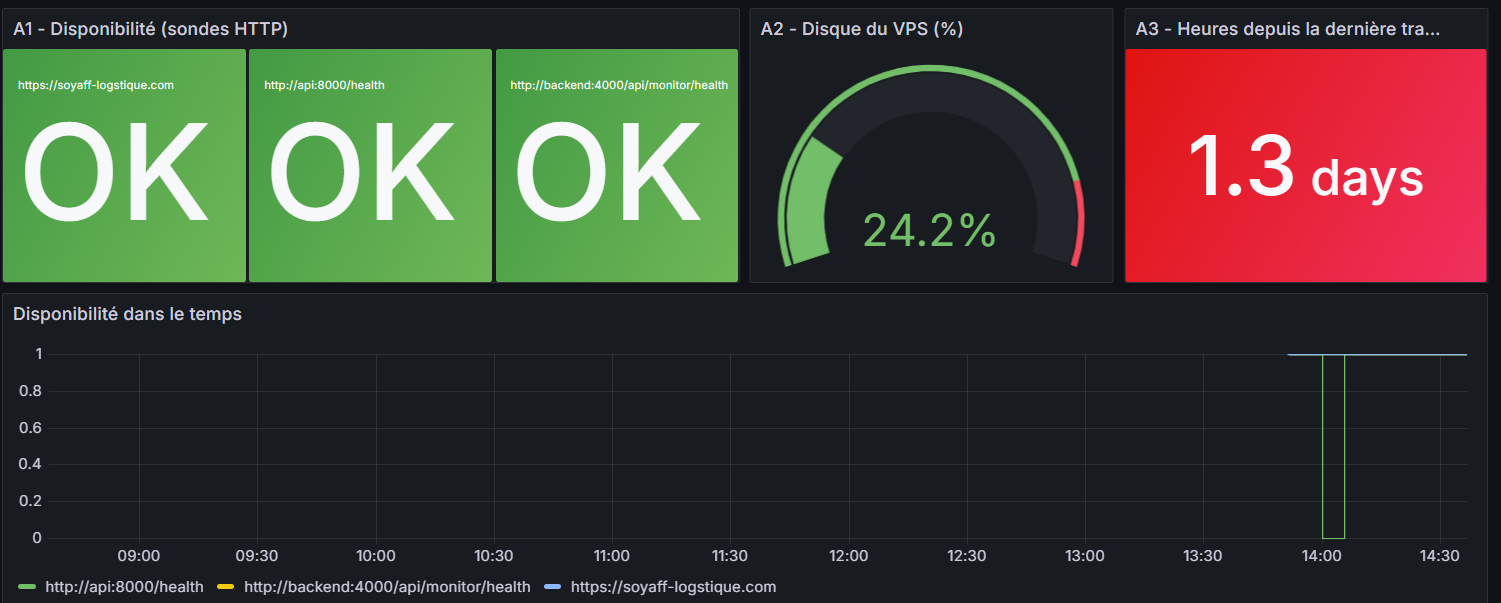
\includegraphics[width=0.85\textwidth]{figures/captures/ops_grafana.png}
    \caption{Tableau de bord Grafana : disponibilité des trois services, disque et fraîcheur des données}
    \label{fig:ops_grafana}
\end{figure}

\begin{figure}[H]
    \centering
    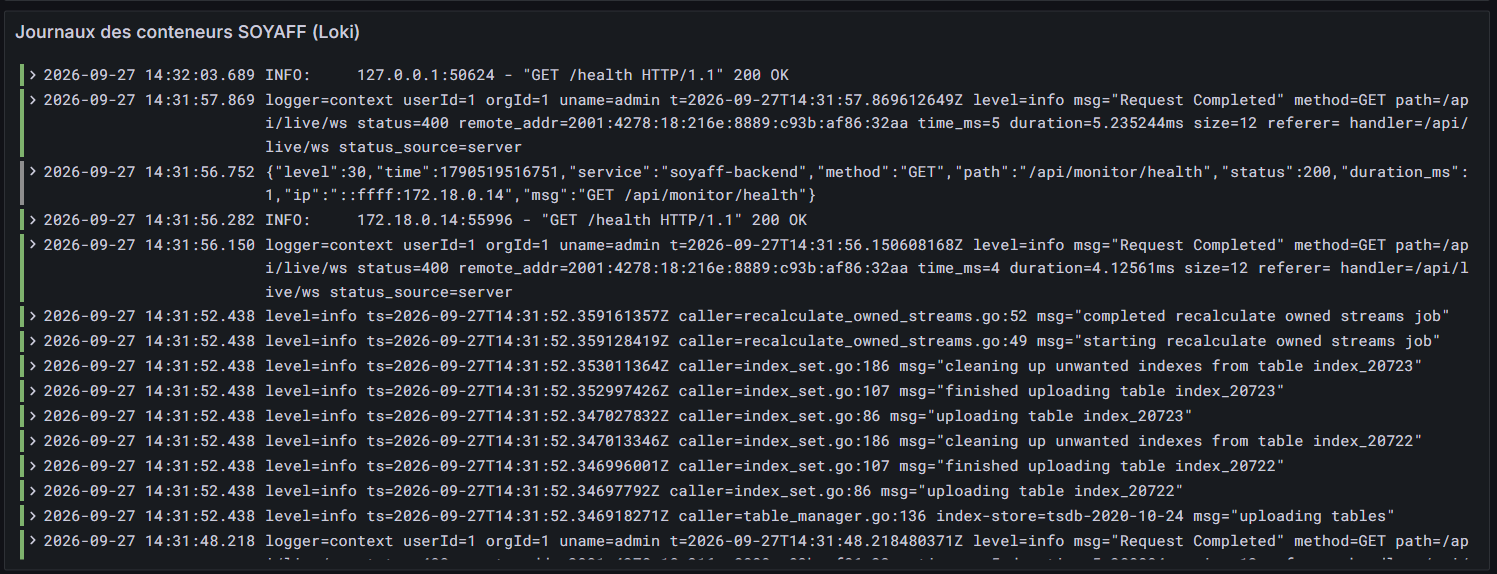
\includegraphics[width=0.85\textwidth]{figures/captures/ops_loki.png}
    \caption{Journaux centralisés des conteneurs dans Loki}
    \label{fig:ops_loki}
\end{figure}

\textbf{Des alertes proactives.} Chaque indicateur porte une règle d'alerte, notifiée sur un canal Telegram par un bot dédié. A1 se déclenche quand un service ne répond plus depuis deux minutes ; A2 quand le disque dépasse 85~\% pendant cinq minutes ; A3 quand aucune transaction n'a été enregistrée depuis plus de 24~heures. Le jeton du bot reste une variable d'environnement, jamais écrite dans le dépôt. Une dégradation n'attend donc plus qu'un utilisateur consulte Grafana pour être connue.

\textbf{Deux pannes provoquées.} Nous avons vérifié ces alertes le 27~septembre~2026 en provoquant deux pannes sur le serveur de production. D'abord, l'arrêt volontaire du service RAG : l'alerte A1 est arrivée sur Telegram à 14:02, puis sa résolution à 14:07 après redémarrage (Figure~\ref{fig:ops_alerte_service}) ; la coupure est visible sur la courbe de disponibilité de la Figure~\ref{fig:ops_grafana}. Ensuite, un fichier temporaire a rempli le disque à 87~\% (Figures~\ref{fig:ops_test_disque_cmd} et~\ref{fig:ops_test_disque_gauge}) : l'alerte A2 est arrivée à 14:33, puis sa résolution après suppression du fichier (Figure~\ref{fig:ops_alerte_disque}).

\begin{figure}[H]
    \centering
    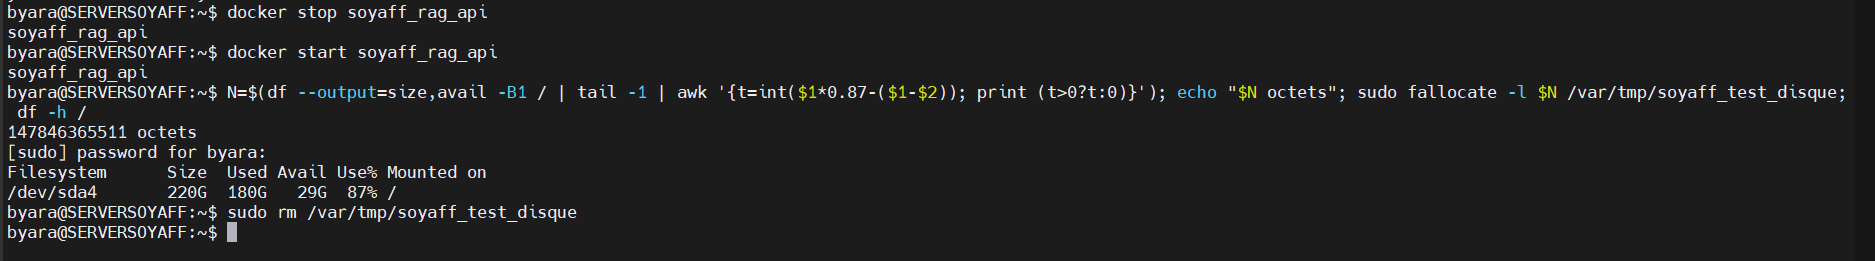
\includegraphics[width=0.9\textwidth]{figures/captures/ops_test_disque_cmd.png}
    \caption{Test de l'alerte disque : arrêt et redémarrage du service RAG, puis remplissage du disque à 87~\%}
    \label{fig:ops_test_disque_cmd}
\end{figure}

\begin{figure}[H]
    \centering
    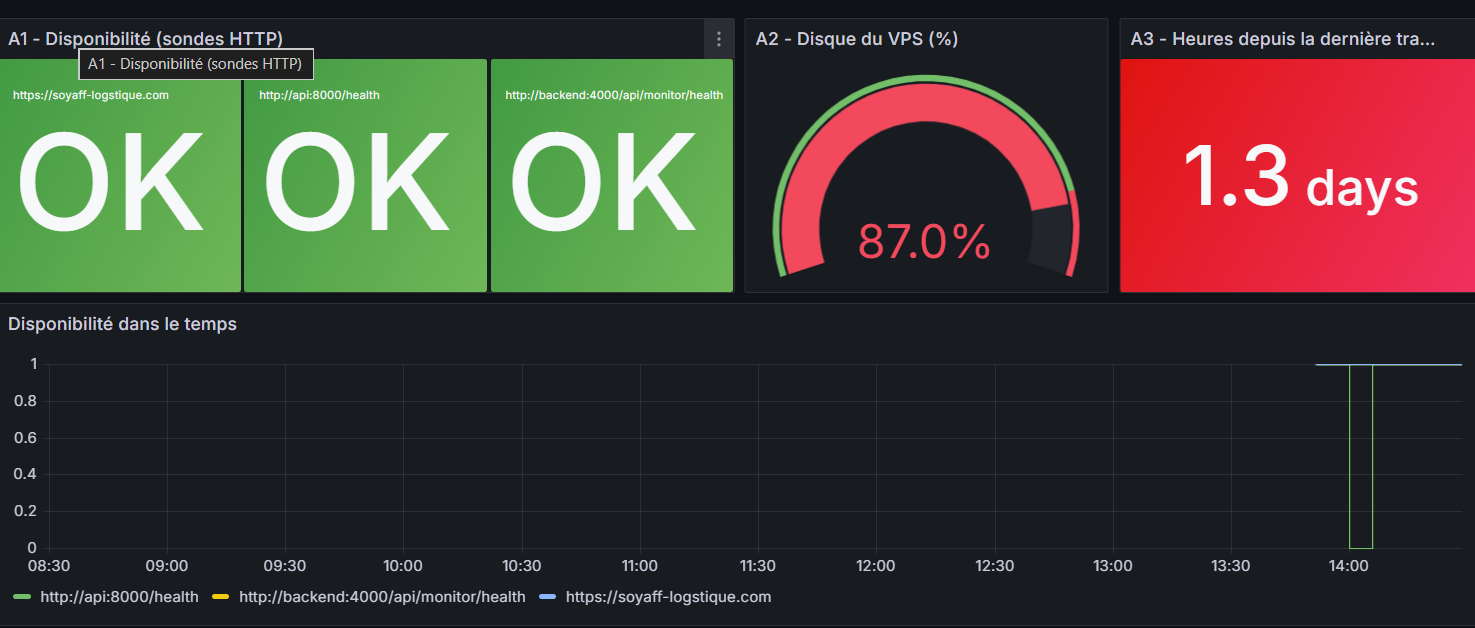
\includegraphics[width=0.7\textwidth]{figures/captures/ops_test_disque_gauge.png}
    \caption{Jauge du disque à 87~\% pendant le test}
    \label{fig:ops_test_disque_gauge}
\end{figure}

\begin{figure}[H]
    \centering
    \begin{minipage}{0.48\textwidth}
        \centering
        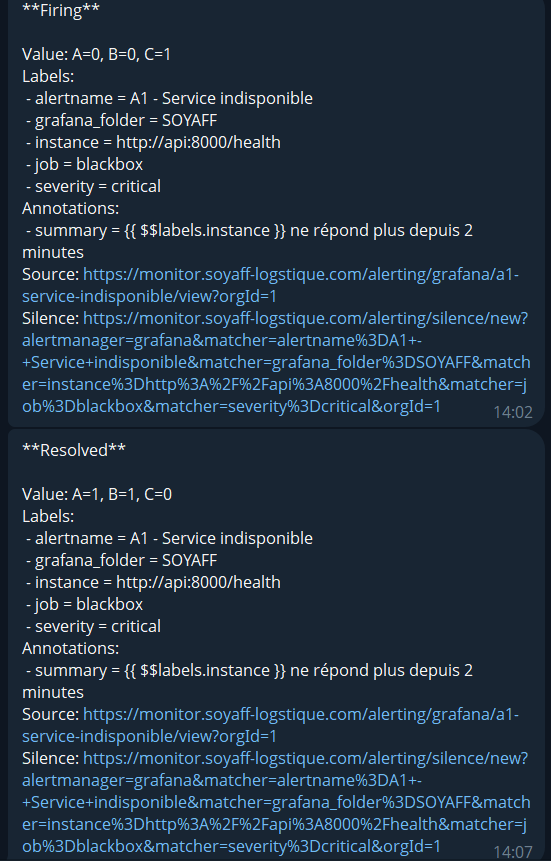
\includegraphics[width=\textwidth]{figures/captures/ops_alerte_service.png}
        \caption{Alerte A1 déclenchée puis résolue (service RAG arrêté)}
        \label{fig:ops_alerte_service}
    \end{minipage}\hfill
    \begin{minipage}{0.48\textwidth}
        \centering
        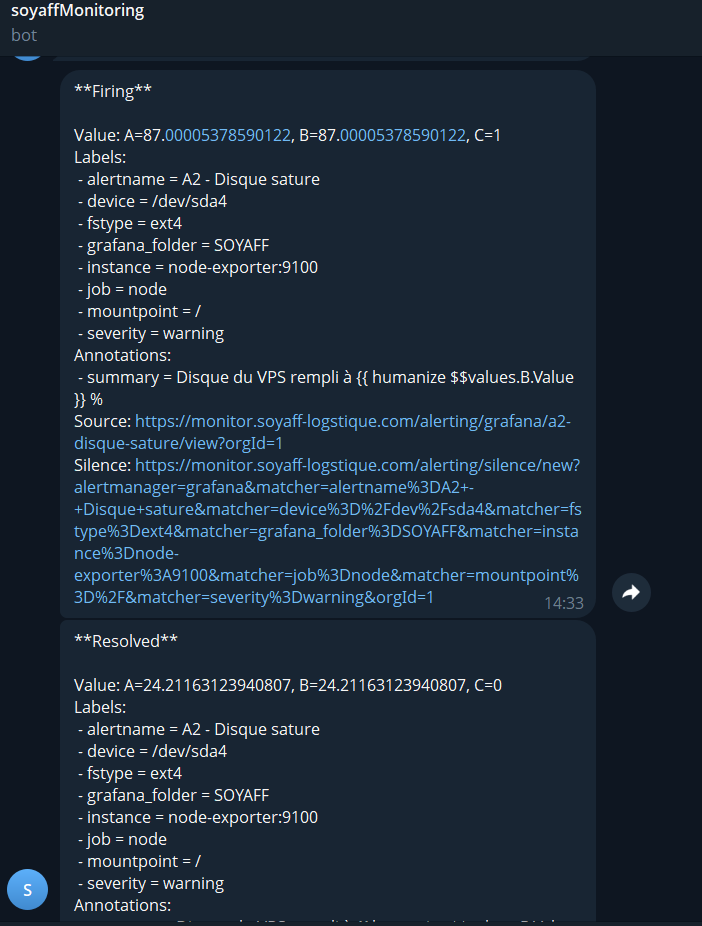
\includegraphics[width=\textwidth]{figures/captures/ops_alerte_disque.png}
        \caption{Alerte A2 déclenchée puis résolue (disque à 87~\%)}
        \label{fig:ops_alerte_disque}
    \end{minipage}
\end{figure}

\textbf{Ce que la supervision couvre.} \texttt{EF-ADM-04} exige de superviser la santé des services ETL, RAG et application web. Les sondes couvrent directement le RAG et l'application ; l'ETL est couvert indirectement par l'alerte de fraîcheur des données, qui ne distingue cependant pas un DAG en échec d'une simple absence de nouveau fichier. \texttt{EF-ADM-04} est donc satisfaite, avec cette réserve pour l'ETL. La même série \texttt{probe\_success} rend la disponibilité (\texttt{ENF-DISP-02}) calculable ; ce calcul relève de la section~\ref{chap:impact_metier}.

\subsection{Sécurité opérationnelle et sauvegarde}
\label{sec:devops_securite}

\textbf{Surface réseau.} Le pare-feu \texttt{UFW} n'ouvre que SSH et les ports~80 et~443 (Figure~\ref{fig:ops_ufw}) ; tous les services sont derrière le Nginx du serveur.

\begin{figure}[H]
    \centering
    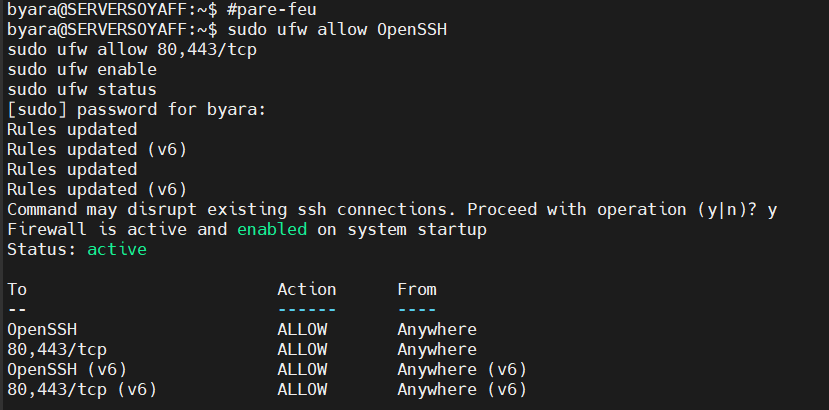
\includegraphics[width=0.55\textwidth]{figures/captures/ops_ufw.png}
    \caption{Pare-feu UFW : seuls SSH, 80 et 443 sont ouverts}
    \label{fig:ops_ufw}
\end{figure}

\textbf{TLS de bout en bout (\texttt{ENF-SEC-05}).} Le trafic des clients passe par Cloudflare. L'ADR-05 avait d'abord retenu le mode \textit{Flexible}, qui laissait en clair le trajet entre Cloudflare et le serveur. Nous sommes passés au mode \textit{Full (strict)} : ce trajet est désormais chiffré lui aussi, et Cloudflare vérifie le certificat du serveur (Figure~\ref{fig:ops_cloudflare}). L'écart à \texttt{ENF-SEC-05} est refermé.

\begin{figure}[H]
    \centering
    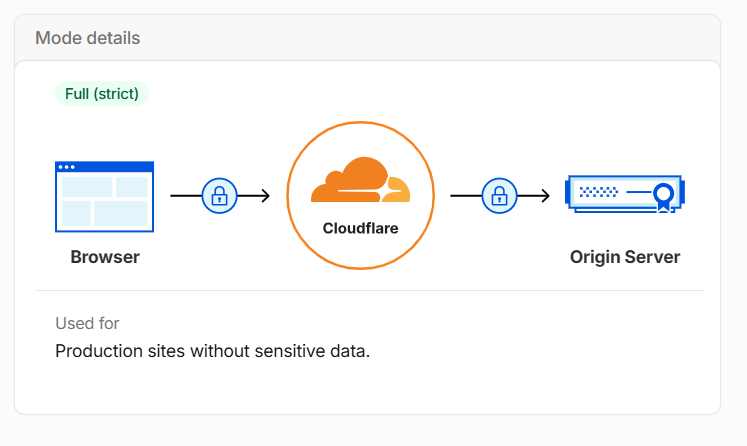
\includegraphics[width=0.45\textwidth]{figures/captures/ops_cloudflare.png}
    \caption{Chiffrement Cloudflare en mode \textit{Full (strict)} : navigateur, Cloudflare et serveur chiffrés de bout en bout}
    \label{fig:ops_cloudflare}
\end{figure}

\textbf{Sauvegarde et restauration (\texttt{EF-ADM-03}, priorité \textit{Must}).} Une tâche planifiée exécute chaque nuit à 02:30 le script \texttt{scripts/backup\_db.sh}. Il produit un \texttt{pg\_dump} de la base, vérifie que l'archive est lisible par \texttt{pg\_restore}, en calcule l'empreinte SHA-256 et conserve quatorze jours d'archives sur le serveur. Il en envoie ensuite une copie hors site, sur l'espace de sauvegarde de 100~Go inclus dans l'offre, par \texttt{rclone} (Figure~\ref{fig:ops_rclone}). Enfin, chaque dimanche à 04:00, une restauration d'essai recharge la dernière archive dans une base jetable, supprimée après vérification. Une sauvegarde jamais restaurée n'est qu'une hypothèse ; celle-ci est éprouvée chaque semaine.

\begin{figure}[H]
    \centering
    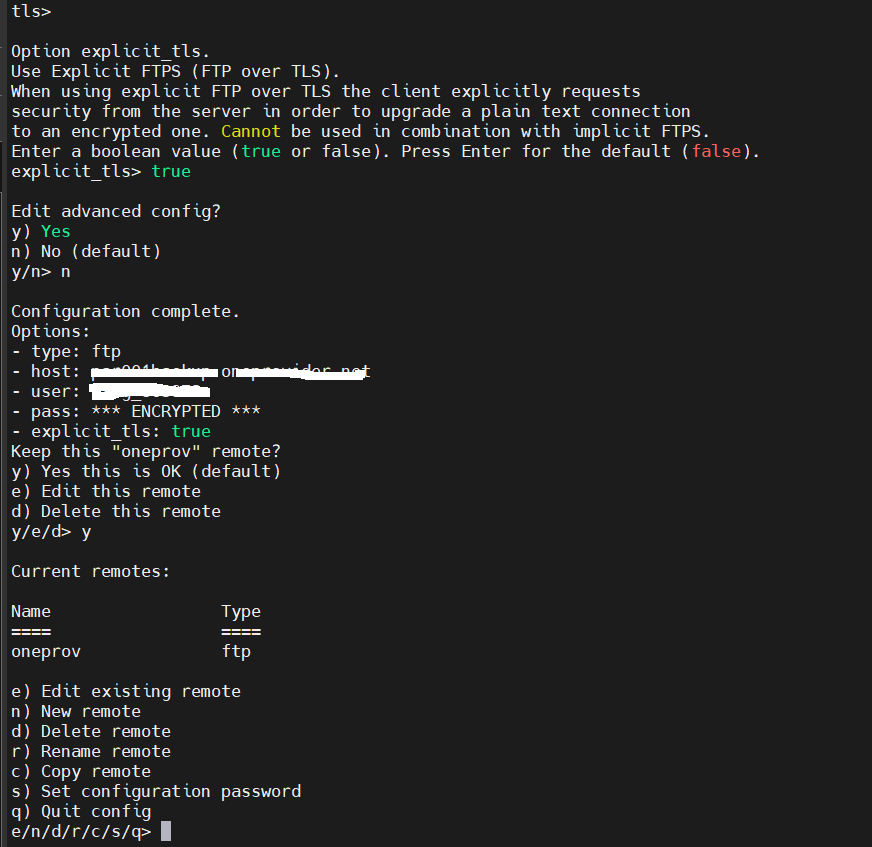
\includegraphics[width=0.45\textwidth]{figures/captures/ops_rclone.png}
    \caption{Configuration de la destination de sauvegarde hors site (\texttt{rclone})}
    \label{fig:ops_rclone}
\end{figure}

\textbf{Piste d'audit.} \texttt{ENF-SEC-04} est satisfaite par la table \texttt{audit\_logs} (section~\ref{chap:webapp}, \S\ref{sec:webapp_rbac}). Les journaux Loki lui sont complémentaires : ils servent l'exploration technique, sans la sémantique métier d'\texttt{audit\_logs}.

\subsection{Écarts, dettes et cohérence}
\label{sec:devops_dettes}

Nous rassemblons ici les écarts du volet DevOps ; leur priorisation est discutée à la section~\ref{chap:discussion}. Ce sont des dettes d'exploitation, pas des défauts de conception : l'infrastructure tient en production, avec des tests bloquants, un déploiement continu, une supervision alertée et une sauvegarde éprouvée.

\begin{itemize}
    \item \textbf{Déploiement sans bascule.} Ni \textit{blue-green}, ni retour arrière automatique ; côté Python, l'échec d'un redémarrage de conteneur ne fait pas échouer le job.
    \item \textbf{Couverture Node non mesurée en CI.} Les tests backend et frontend bloquent le pipeline, mais leur couverture n'est pas calculée, alors que le plancher de 70~\% est déjà déclaré dans \texttt{jest.config.cjs}.
    \item \textbf{\textit{Runner} en mode \texttt{shell}.} Les jobs s'exécutent directement sur le serveur de production, sans isolation par conteneur.
    \item \textbf{Copie hors site non chiffrée.} La base contient des données personnelles (table \texttt{chauffeurs}) ; la copie envoyée sur l'espace FTP de l'hébergeur passe en TLS mais y est stockée en clair. Un chiffrement côté client (\texttt{rclone crypt}) est déjà prévu par le script.
    \item \textbf{Configuration Nginx hors dépôt.} Le Nginx du serveur, qui route les sous-domaines, n'est versionné nulle part.
    \item \textbf{Copie de sauvegarde non chiffrée.} L'archive envoyée hors site contient des données personnelles et n'est pas encore chiffrée.
    \item \textbf{Point de défaillance unique} (ADR-03), inchangé.
\end{itemize}

Plusieurs dettes relevées lors de la première rédaction sont refermées. Le TLS est chiffré de bout en bout (\textit{Full (strict)}). La supervision, autrefois passive, envoie des alertes. La sauvegarde, autrefois absente malgré sa priorité \textit{Must}, est quotidienne, copiée hors site et restaurée chaque semaine. La suite \texttt{pytest}, dont le résultat était masqué, bloque désormais le pipeline avec un plancher de couverture de 95~\%. La pile de supervision est versionnée. S'y ajoutent deux résorptions plus anciennes : la migration de PostgreSQL~13 vers~16 et le passage de l'image \texttt{api} à Python~3.11 sous un utilisateur non-\textit{root}.

\subsection{Synthèse et transition}
\label{sec:devops_synthese_transition}

Nous avons décrit dans cette section la chaîne DevOps qui porte les modules des sections~\ref{chap:etl}, \ref{chap:webapp} et~\ref{chap:ia_rag} : conteneurisation mono-hôte frugale (\S\ref{sec:devops_conteneurisation}), intégration et déploiement continus avec des tests bloquants (\S\ref{sec:devops_cicd}), supervision par sondes, métriques, journaux et alertes (\S\ref{sec:devops_observabilite}), sécurité et sauvegarde (\S\ref{sec:devops_securite}). Les écarts restants (\S\ref{sec:devops_dettes}) bornent ce que l'infrastructure garantit sans remettre en cause la plateforme.

Le chapitre se referme sur une plateforme construite, déployée et exploitée : un pipeline qui consolide les données historiques, une application web qui les expose sous contrôle d'accès, un module conversationnel hybride qui les interroge sans exposer les données sensibles, et l'infrastructure qui porte l'ensemble avec des ressources limitées. Le chapitre~\ref{chap:evaluation} la soumet maintenant à l'épreuve des faits, hypothèse par hypothèse.
